\chapter{How to Write Descriptively}

この講義は、読者の側から始まり、それから craft の側へ向きを変える。私たちはまず、なぜ fiction が重要なのかを問う。ついで、それが lived experience や theater や film と同じほど強く私たちを absorb するためには、prose が何をしなければならないのかを問う。中心的な主張は、descriptive language は story の上に載せられた decoration ではない、ということだ。それは、ページ上の static な marks が sensation、association、そしてついには immersion へと変わる、その mechanisms の一つなのである。

\section{なぜ私たちは fiction を読み、なぜ description が重要なのか}

冒頭の list は、意図的に broad である。私たちは entertainment のために fiction を読み、誰がやったのかを知るために読み、strange new worlds へ travel するために読み、怖がるために、笑うために、泣くために、考えるために、感じるために読む。だが講義は、motive の catalogue に私たちを置いたままにはしない。もっとも強いものへと drive していく。すなわち、私たちは、しばらくのあいだ自分がどこにいるかを忘れるほど absorb されるために読むのだ、ということである。これが、後に続く craft advice のすべてを judge する standard になる。
\begin{equation}
\text{fiction} \Rightarrow \text{absorption / immersion}.
\end{equation}

\begin{definition}
Immersion とは、読者が story world について merely informed されるのではなく、その内部に present していると feel する、一時的な spell のことである。
\end{definition}

この standard が fixed されると、講義は direction を reverse する。もし fiction が私たちに対してこれをするのだとしたら、それをどうやってページの上で起こすのか。講師は、familiar な candidates を quick succession で test する。exciting な plot だろうか。おそらくそうだ。fascinating な characters だろうか。たぶんそうだ。beautiful な language だろうか。これもおそらくそうだ。圧縮すれば、
\begin{equation}
\text{reader engagement} \leftarrow \{\text{plot},\ \text{character},\ \text{language}\}.
\end{equation}
となる。この triad の point は、plot や character を deny することにはない。講義が本当に問いかけたい question への道を clear することにある。どのような kind の language が、prose を experience へと変えるのか。

\subsection{Question \& Answer}

\paragraph{Question.} fiction がページの上で私たちを hold したいなら、何をしなければならないのか。

\paragraph{Answer.} それは、events を report する以上のことをしなければならない。reader が imaginatively に story の中へ relocate されるような state を create しなければならないのである。講義はこの demand から始まることで、description を literary ornament ではなく、functional necessity として扱えるようにしている。

\section{metaphor と flat な statement}

講師は、abstract に答えない。ひとつの sentence を私たちの前に置き、それを test する。Billy の legs は noodles であり、her hair の ends は poison needles であり、her tongue は bristly sponge であり、her eyes は bags of bleach である。そしてそこに check が入る。これで私たちは almost Billy と同じくらい queasy に feel しただろうか。完全にではない。だが plain な statement よりは、そこへずっと近づく。

この local comparison は、
\begin{equation}
\text{metaphorical description} > \text{flat paraphrase},
\end{equation}
と書ける。ここで \(>\) が意味するのは numerical superiority ではなく、greater vividness である。講義はすぐにその why を説明する。Billy の legs が literally noodles なのではない。その line は implied comparison によって work している。bodily state を、reader が partially simulate できる sensory terms へ translate しているのだ。もしこの sentence を ``Billy feels nauseated and weak'' へ flatten してしまえば、information は preserve される。だが pressure は失われる。

この distinction は、次のように書くとさらに sharp になる。
\begin{equation}
\text{understanding} \neq \text{feeling}, \qquad
\text{reading} \neq \text{immersion}.
\end{equation}
人は Billy の condition を understand しながら、なおその外側に remain していられる。description が matter し始めるのは、まさに paraphrase が届かなくなるその地点においてである。

\subsection{Question \& Answer}

\paragraph{Question.} なぜ metaphorical な version のほうが、literal な paraphrase より強く feel されるのか。

\paragraph{Answer.} metaphor は、Billy の state を merely classify するのではなく、それを bodily かつ sensory な terms に recode するからである。paraphrase が与えるのは diagnosis であり、metaphor が与えるのは participation により近いものだ。

\section{static symbols から成る sensory medium としての prose}

Billy の example から、講義は theory へ widen していく。fiction は、私たちに spell をかける、と言われる。story の world の中に自分が living しているという momentary illusion である。その spell は senses に依存している。good prose は、characters が undergoing していることの vivid な mental simulacra を build することを私たちに help する。

ここで講師は、prose を stage や screen と contrast させる。theater と film は、いくつかの senses を directly engage する。gesture、setting、movement が見え、voices、noise、atmosphere が聞こえる。prose の task は、もっと hard である。なぜなら、それは contrasting background の上の inert な marks から始まるからだ。
\begin{align}
\text{stage/screen} &\to \text{direct sensory presentation},\\
\text{prose} &\to \text{static symbols} \to \text{constructed experience}.
\end{align}
その consequence は、ただちに follow する。もし prose が matter-of-fact で non-tactile のままであれば、その spell は thin になる。
\begin{align}
\text{matter-of-fact language} &\Rightarrow \text{weak spell} \Rightarrow \text{immersion より interpretation},\\
\text{well-chosen language} &\Rightarrow \text{vivid mental simulacra}.
\end{align}
この mechanism は、もう一段 explicit に summarizing できる。
\begin{equation}
\text{static symbols} \to \text{sensory cues} \to \text{mental simulacra} \to \text{immersion}.
\end{equation}

ここでの講義の point は exact である。prose は directly show することができない。ゆえに indirectly trigger しなければならない。だからこそ description がこれほど重要になる。それは、medium が見かけ上もつ poverty を language が compensate する場所の一つなのである。

\subsection{Question \& Answer}

\paragraph{Question.} prose が symbols しか与えないのなら、どうして felt experience を create できるのか。

\paragraph{Answer.} それらの symbols を、conceptual recognition で止まらないように arrange することによってである。それらは hearing、touch、motion、sight、smell、taste を awaken し、それからそれらを coherent な imaginative state へ bind しなければならない。prose は sensation を deliver しない。それを elicit するのである。

\section{``Ghost Quiet'' の close reading}

general な mechanism が置かれると、講義はひとつの sentence に pause し、それを carefully に読む。
\[
\text{``The world was ghost quiet, except for the crack of sails and the burbling of water against hull.''}
\]
sentence が unpack される前に、講師は、fiction が operate する sensory field に name を与える。
\begin{equation}
\{\text{taste},\ \text{smell},\ \text{touch},\ \text{hearing},\ \text{sight},\ \text{motion}\}.
\end{equation}
だがこの sentence は、senses に touch する以上のことをしている。それは conceptual association も create している。その line の force は、その combination にある。

講師の layered reading を faithful に reconstruction すれば、
\begin{align}
\text{description} &= \text{hearing} + \text{motion/touch} + \text{metaphoric association},\\
\text{hearing} &= \text{quiet} + \text{crack} + \text{burbling},\\
\text{motion/touch} &= \text{sails} + \text{water against hull},\\
\text{metaphoric association} &= \text{ghost}.
\end{align}
となる。第一の layer は auditory である。講師は明示的に、この sentence が generic な word ``sound'' を使っていないと note する。代わりに、それは shape と texture をもつ words を使っている。``Crack'' と ``burbling'' は、単に acoustic event に name を与えるだけではない。その quality を specify するのである。

それから別の layer が laid down される。sails は motion を imply し、water against the hull は contact、pressure、surface を imply する。最後に ``ghost'' が ``quiet'' を modify し、それでもなお sentence の felt atmosphere に属している abstract relation を introduce する。だからこそ、より大きな relation を書く価値がある。
\begin{equation}
\text{sensory engagement} + \text{abstract association} \to \text{richer description}.
\end{equation}

\begin{figure}[h]
\centering
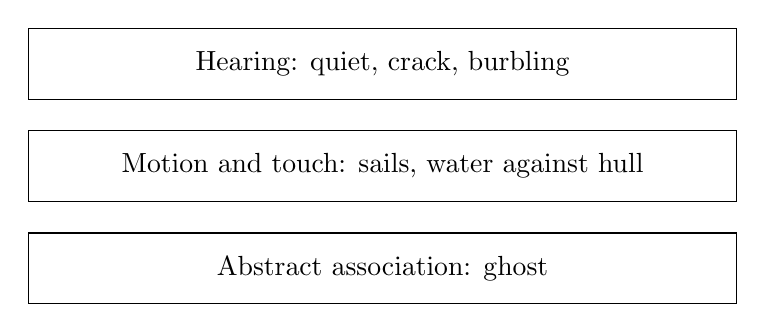
\begin{tikzpicture}
\node[draw, rectangle, minimum width=9cm, minimum height=0.9cm] (A) at (0,1.8) {Hearing: quiet, crack, burbling};
\node[draw, rectangle, minimum width=9cm, minimum height=0.9cm] (B) at (0,0.5) {Motion and touch: sails, water against hull};
\node[draw, rectangle, minimum width=9cm, minimum height=0.9cm] (C) at (0,-0.8) {Abstract association: ghost};
\end{tikzpicture}
\end{figure}

この transcript-based の schematic は、意図的に simple である。講義自身が sentence を unfold していく order を record している。まず sound、ついで movement と contact、そして最後に、line 全体の atmosphere を変える abstract modifier である。

\paragraph{Worked example.} analytic order は重要である。
\begin{enumerate}
\item sound-words を isolate する。``quiet,'' ``crack,'' ``burbling.''
\item これらが generic な class ではなく、specific な acoustic qualities であることを observe する。
\item それから sails と water against hull を通して motion と touch を register する。
\item そのあとではじめて、quiet と ghost のあいだの abstract な link を take in する。
\item sentence が work するのは、これらの layers が互いの代わりになるのではなく、accumulate するからである。
\end{enumerate}

\subsection{Question \& Answer}

\paragraph{Question.} ひとつの sentence は、どうやって複数の sensory と conceptual の layers を accumulate するのか。

\paragraph{Answer.} words がみな同じ function に serving しているのではないからである。あるものは sound を sharpen し、あるものは movement や contact を imply し、あるものは nonliteral な association を create する。strong な descriptive sentence は、その labor を several registers に distribute し、それらの registers に互いを reinforce させる。

\section{metaphor、simile、そして読者との distance}

次の step は、この講義でもっとも precise なものの一つである。講師は、``ghost quiet'' を praise するだけではない。それを近接した alternative と contrast させる。``quiet as a ghost.'' この difference は、単に grammatical なのではない。それは、scene に対する reader の relation を change する。
\begin{align}
\text{quiet as a ghost} &\Rightarrow \text{greater distance},\\
\text{ghost quiet} &\Rightarrow \text{greater immediacy}.
\end{align}
この formal distinction は、
\begin{align}
\text{simile} &\to \text{overt comparison},\\
\text{metaphor} &\to \text{implied comparison}.
\end{align}
と書ける。

この claim は local に keep しておくべきである。講義は、metaphor が simile を always outrank すると prove しているのではない。この instance において、simile が extra の interpretive layer を insert してしまうことを示しているのだ。私たちは、how to compare をもっと openly に told されることになる。そして、その explicitness は私たちを experience の slightly outside で pause させてしまう。``Ghost quiet'' は、terms をより tightly に fuse する。comparison は、上から announce される代わりに、phrase の内部で起こるのである。

これが、講師の言う distance の意味である。一方の formulation は、その relation を inspect させる。他方の formulation は、私たちをそこへより quickly に inhabit させる。

\subsection{Question \& Answer}

\paragraph{Question.} simile は何を add し、どのような distance を impose するのか。

\paragraph{Answer.} simile は explicitness を add する。comparison を unmistakable にするのだ。それは useful でありうるが、ここでは immediacy を weaken する。reader を sensation から一歩 farther に置いてしまうからである。metaphor は comparison を implied のままにし、scene をより immediate に保つ。

\section{clich\'e に抗して: fresh な connotation と reader participation}

講義はいま、metaphor と simile の local な distinction から、より broad な problem へ向かう。clich\'e である。writers は overused images を avoid するよう told される。そして講義は、その advice に real な content を与える。
\begin{equation}
\text{overused image} \Rightarrow \text{low reader engagement}.
\end{equation}
``red as a rose'' のような phrase は、ほとんど何も demand しない。comparison は、すでに processed されたものとして arrive してくる。reader は十分な imaginative work をするよう求められていないのである。

counterexample も同じく exact である。``stewed cherry dress'' という phrase が与えられる。この phrase は、complete なものとして arrive しない。color、texture、density、さらには atmosphere までも reader に infer させる。image は obscure なのではない。active なのである。したがって、講義の final relation は
\begin{equation}
\text{unexpected connotation} \to \text{reader participation} \to \text{immersion}.
\end{equation}
となる。reader は、もはや merely description を receiving しているのではない。scene を build する手助けをしているのである。

だからこそ講義は、theory ではなく prescription で閉じる。sound、sight、taste、touch、smell、movement を engage するような、well-chosen words を使いなさい。そして story の elements のあいだに unexpected connotations を create しなさい。最後の compression は、
\begin{equation}
\text{sensory cue} + \text{fresh association} \Rightarrow \text{dynamic imaginative world}.
\end{equation}
となる。reader の brushfire imagination に火をつける、という phrase は ornamental flourish ではない。それは argument の endpoint なのである。description が succeed するのは、reader を observer から participant へ変えるときだ。

\section{まとめ}

講義は strict な sequence で move する。私たちはまず、なぜ fiction を読むのかという問いから始め、immersion を governing standard として得る。それから、prose がどうやってその standard を achieve できるのかを問い、その answer を Billy の example に対して test する。そこでは vivid な metaphor が flat な summary よりも stronger であることが証明される。そこからさらに、static symbols の medium でありながら nevertheless sensory experience を produce しなければならないものとしての prose の theory へ widen する。そして、world が ``ghost quiet'' であったという sentence が、この講義における layered description の worked example になる。hearing、motion、touch、abstraction が single line の中に assemble されている。最後に講義は、metaphor と simile を、それぞれが create する distance の degree によって distinguish し、clich\'e に警告を発し、fresh な connotation がなぜ reader の imagination を scene の making に recruit するのかを示す。その result は、severe でありながら practical な lesson である。description は、fiction が language を lived experience へ変える、その場所の一つなのである。